\chapter{Introduction}
\label{chp:introduction}


%%%%%%%%%%%%%%%%%%%%%%%%%%%%%%%%%%%%%%%%%%%%%%%%%%%%%%%%%%%%%%%%%%%%%%%
\section{Problem Statement}

In this report a feedback control system for a robotic gymnast that is able to swing from the "hanging" position to the "handstand" position will be designed, implemented and verified. Feedback control loops must be designed that use the "legs" of the gymnast to swing the "body" of the gymnast from the "hanging" position to a "handstand" position and then balance the gymnast on top of the horizontal bar. A mathematical model for the dynamics of the swinging robotic gymnast system must be derived or sourced from literature. The dynamics are analysed to propose an appropriate feedback control architecture that actuates the "legs" of the gymnast using feedback from sensors that measure the swinging motion of the gymnast on a horizontal bar. A practical demonstrator must be constructed and the correct operation must be demonstrated.\\

\section{The Robotic Gymnast System}
\begin{figure}[h]
	\centering
	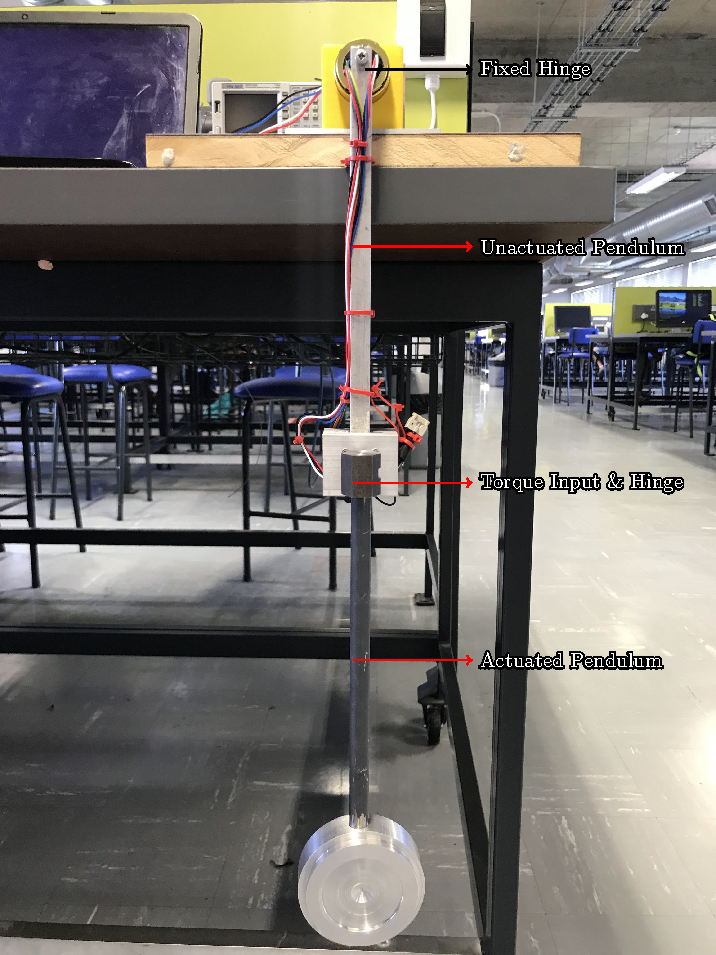
\includegraphics{./figs/overview/overview.pdf}
	\caption{Overview of the Robotic Gymnast System}
	\label{fig:overview}
\end{figure}

Figure \ref{fig:overview} provides an overview of the robotic gymnast system to create a mental picture for the variables and concepts used throughout the report. There are 2 pendulums that are attach together with a hinge. At this hinge there is a torque being applied by a motor to the actuated pendulum. The entire system rotates around the fixed hinge at the top to which the unactuated pendulum is connected. The system is describe using two independent parameters, $\theta$ and $\phi$. $\theta$ described the response of the unactuated pendulum whereas $\phi$ describes the behaviour of the actuated pendulum relative to $\theta$.\\

The goal is to use the feedback of the independent parameters to apply a torque to the actuated pendulum to swing the gymnast from the hanging position and balance in the inverted position. This is accomplished by using a microcontroller to interface with sensors to provide information about the independent parameters and implement the control laws in software.\\


\section{Literature Study}
\label{sec:literature_study}
% WHAT you are going to present in this chapter/section
% WHY you are presenting it, and
% HOW you are going to present it
\begin{comment}
	Previous approaches used to control an underactuated system is to use the intrinsic dynamics of the system to attain the desired behaviour \citep{tedrake}. This leads to the approach to exploit the dynamics of the system by using the 'legs' of gymnast to swing.\\
\end{comment}	

A literature study was performed to survey different physical implementations of the system, different approaches to modelling the dynamics, different physical implementations of the system, and different techniques to perform the feedback control to perform the swing-up and the balancing of the robotic gymnast.\\

Previous attempts to swing up and balance the robotic gymnast used two separate controllers. The first controller is responsible for swinging the robotic gymnast from the hanging position up towards the inverted position. When the swing-up controller brought the gymnast near the inverted position, a new controller is used to balance the gymnast. The different types of swing up and balancing controllers used by previous researchers are summarised below, followed by a decision on the approaches selected for this project.\\

\citet{spong_swingup} implemented the swing-up controller by using partial feedback linearisation which results in a linear response from either the \textit{actuated} or \textit{unactuated} pendulum. Using \textit{non-collocated} linearisation he was able to control the \textit{unactuated} pendulum to follow a desired trajectory. \citeauthor{spong_swingup} used the phase portrait of the zero dynamics of the system to show that the closed-loop system will converge to the inverted equilibrium position. \citeauthor{spong_swingup} also demonstrated how the swing-up can be achieved by using \textit{collocated} linearisation which linearises the response of the \textit{actuated} pendulum. This allows the actuated pendulum to follow a desired trajectory and \citeauthor{spong_swingup} provides a energy-based trajectory that increases the energy in the system. Once both swing up controller brings the system to the inverted balancing position, the feedback control system switches over to a linear quadratic regulator (LQR) to balance the system.\\

\citet{Brown1997} provided two manually tuned nonlinear controllers for the balancing of the robotic gymnast and tested and compared them against a designed LQR controller. The two nonlinear controllers were a direct fuzzy controller (DFC) and a fuzzy model reference learning controller (FMRLC). The gains for the DFC controller were based on the gains of the LQR controller. The DFC controller was implemented and successfully balanced the gymnast. However the LQR controller provided smoother state trajectories and smaller control input. The FMRLC uses no explicit dynamical reference model and instead the outputs of the plant using normalising gains are directly fed into the second fuzzy system. The FMRLC controller was a significant improvement on the DFC, but yet again did not perform as well as the LQR controller.\\


\citeauthor{Brown1997} also attempted to swing the robotic gymnast to the inverted balancing position using the energy based trajectory proposed by \citeauthor{spong_swingup}, but without the partial linearisation feedback. \citeauthor{Brown1997} were able to swing and balance the robotic gymnast using this approach, but their approach resulted in larger input signals that were not as smooth as the input signals when using partial feedback linearisation.\\



In most of the literature, the mathematical model of the robotic gymnast is derived using the Euler-Lagrangian equation. This approach is used because the mechanical energy in the system is easily identified. \citet{derivation_controlPlaner} and \citet{tedrake} both derived the simplified mathematical models for the robotic gymnast using point mass approximations. \\

Based on the literature study, it was decided to perform the swing up control using partial feedback linearisation and an energy-based reference trajectory. The balancing controller was decided to be a linear full state feedback controller.


\begin{comment}


The ordinary differential equations (ODE's) describing a system can be arranged as a set of linear differential equations. Describing a system in such a way is known as the State Space design approach, where the solution is the trajectory of the chosen state variables.\cite{textbook}

These ODE's are required to be written as vectors in the state-variable form seen in equation (\ref{eq:statespace1}) and (\ref{eq:statespace2})
\begin{equation} \label{eq:statespace1}
\centering
\boldsymbol{\dot{x}} = \boldsymbol{A}\boldsymbol{x} + \boldsymbol{B}u
\end{equation}
\begin{equation} \label{eq:statespace2}
\centering
\boldsymbol{y} = \boldsymbol{C}\boldsymbol{x} + Du
\end{equation}
The \textit{n}th-column vector $\boldsymbol{x}$ is called the state of the system for a \textit{n}th-order system. The \textbf{A} matrix is the system matrix, containing \textit{n}$\times$\textit{n} elements and the input matrix is the \textit{n}$\times 1$ \textbf{B} matrix. \textbf{C} is a $1\times$\textit{n} row matrix called the output matrix and the scalar D is known as the direct transmission term \cite{textbook}.

A system parameter of great interest to control engineers are the poles of the system. It provides the characteristic response of the system starting at a initial condition with no forcing function. These poles,\textbf{s}, are the natural frequencies of the system and the state space representation allow these poles to be easy identified. The poles are the solution to the eigenvalue problem of the \textbf{A} matrix shown in equation (\ref{eq:statespace_eigen}) \cite{textbook}.
\begin{equation} \label{eq:statespace_eigen}
\centering
\text{det}(s\boldsymbol{I} - \boldsymbol{A}) = 0
\end{equation}

The poles of the system can be assigned new positions to satisfy dynamic response specification by introducing feedback. The feedback is a linear combination of the state variables $\boldsymbol{x}$ resulting in the input of the system $u$ to be transformed as seen in equation (\ref{eq:feedbackgain}) and represented in Figure \ref{fig:linearSys}. Substituting equation (\ref{eq:feedbackgain}) into (\ref{eq:statespace1}) the characteristic equation is now describe as (\ref{eq:closedSysFeedback}). The corresponding characteristic equation is: $$\alpha_{s}=(s-s_{1})(s-s_{2})\ldots(s-s_{n}) $$ This shows by selecting the correct gain matrix \textbf{K} the poles of the system can be moved to a desired position.
\begin{equation} \label{eq:feedbackgain}
\centering
u = -\boldsymbol{K}\boldsymbol{x}
\end{equation}

\begin{figure}
	\centering
	% System Combination
% Harish K Krishnamurthy <www.ece.neu.edu/~hkashyap/>
\documentclass{article}

\usepackage{tikz}
\usetikzlibrary{shapes,arrows,shadows}
\usepackage{amsmath,bm,times}
\newcommand{\mx}[1]{\mathbf{\bm{#1}}} % Matrix command
\newcommand{\vc}[1]{\mathbf{\bm{#1}}} % Vector command

\begin{document}
	% Define the layers to draw the diagram
	\pgfdeclarelayer{background}
	\pgfdeclarelayer{foreground}
	\pgfsetlayers{background,main,foreground}
	
	% Define block styles used later
	
	\tikzstyle{sensor}=[draw, fill=blue!20, text width=5em, 
	text centered, minimum height=2.5em,drop shadow]
	\tikzstyle{ann} = [above, text width=5em, text centered]
	\tikzstyle{wa} = [sensor, text width=10em, fill=red!20, 
	minimum height=6em, rounded corners, drop shadow]
	\tikzstyle{sc} = [sensor, text width=13em, fill=red!20, 
	minimum height=10em, rounded corners, drop shadow]
	
	% Define distances for bordering
	\def\blockdist{2.3}
	\def\edgedist{2.5}
	
	\begin{tikzpicture}
	\node (wa) [sensor]  {$\boldsymbol{\dot{x}}= \boldsymbol{A}\boldsymbol{x}+\boldsymbol{B}$};
	\path (wa.south)+(0,-1) node (feedback) [sensor] {$u = -\boldsymbol{K}\boldsymbol{x}$};
	
	\path (wa.east)+(\blockdist/1.5,0) node (C) [sensor] {$\boldsymbol{C}$};
	\path (C.east)+(\blockdist/1.5,0) node (Y) [sensor] {$\boldsymbol{y}$};
	
	
	\path [draw, ->,thick] (wa.east) -- node [above] {} 
	(C.west);
	
	\path [draw, ->,thick] (C.south) |- node [above] {} 
	(feedback.east);
	
	\path [draw, ->,thick] (C.east) -- (Y.west);
	
	\path [draw, ->,thick] (feedback.west) -| ([xshift=-1cm]wa.west) -- (wa.west) {};
	
	%\path [draw, ->,] (C.east) -- node [above] {} 
	%	(Y.west);
	
	%\path (wa.south) +(0,-\blockdist) node (asrs) {System Combination - Training};
	
	%\begin{pgfonlayer}{background}
	%   \path (asr1.west |- asr1.north)+(-0.5,0.3) node (a) {};
	%  \path (wa.south -| wa.east)+(+0.5,-0.3) node (b) {};
	% \path (C.east |- asrs.east)+(+0.5,-0.5) node (c) {};
	
	%\path[fill=yellow!20,rounded corners, draw=black!50, dashed]
	%   (a) rectangle (c);           
	% \path (asr1.north west)+(-0.2,0.2) node (a) {};
	
	%\end{pgfonlayer}
	
	\end{tikzpicture}
	
\end{document}}
	\caption{State Space Representation with Feedback Gain}
	\label{fig:linearSys}
\end{figure}

\begin{equation} \label{eq:closedSysFeedback}
\centering
\text{det}[s\boldsymbol{I}-(\boldsymbol{A}-\boldsymbol{B}\boldsymbol{K})] = 0
\end{equation}

The classical approach to controlling a system is by implementing a controller which reacts on the error of the desired state and the current state. These controllers are more commonly known as PID-controllers where the controller equation is shown in (\ref{eq:PID}).

\begin{equation} \label{eq:PID}
\centering
u(t) = K[ e(t)+K_{I}\int_{0}^{t}e(\tau)d\tau +K_{D}\frac{de(t)}{dt}]
\end{equation}

Each term represent an effect it has on the system response when the PID-controller is implemented shown in Figure \ref{fig:PIDcontroller}. If the system or plant is assumed to be a second-order differential equation represented by:
\begin{equation} \label{eq:PID_system}
\centering
\dddot{q}+(2\zeta\omega_{n}+K_{D})\ddot{q}+(\omega_{n}^2+K_{P})\dot{q}+K_{I} = 0
\end{equation}

From equation (7) it is visible that by tuning the PID constants the response of the system can controlled.
\end{comment}


\section{System Overview}
\label{sec:system_overview}
%WHAT you are going to present in this chapter/section
%WHY you are presenting it, and
%HOW you are going to present it
\begin{figure}[h]
	\centering
	\newcommand{\mx}[1]{\mathbf{\bm{#1}}} % Matrix command
\newcommand{\vc}[1]{\mathbf{\bm{#1}}} % Vector command


% Define the layers to draw the diagram
\pgfdeclarelayer{background}
\pgfdeclarelayer{foreground}
\pgfsetlayers{background,main,foreground}

% Define block styles used later

\tikzstyle{sensor}=[draw, fill=red!20, text width=5em, 
text centered, minimum height=2.5em,drop shadow,rounded corners]
\tikzstyle{ann} = [above, text width=5em, text centered]
\tikzstyle{wa} = [sensor, text width=10em, fill=red!20, 
minimum height=6em, rounded corners, drop shadow]
\tikzstyle{sc} = [sensor, text width=13em, fill=red!20, 
minimum height=10em, rounded corners, drop shadow]

% Define distances for bordering
\def\blockdist{2.3}
\def\edgedist{2.5}

\begin{tikzpicture}[scale=1.2]
\centering
\node (wa) [wa]  {\textbf{Electronic Design} \\ PCB \\ Signal Conditioning};
\path (wa.west)+(-\blockdist,0) node (asr1) [wa] {\textbf{External Computer} \\ Controller \\ Data Aquisition };
\path (wa.east)+(\blockdist,0) node (vote) [wa] {\textbf{Mechanical Design} \\ State variables \\ };
\path (wa.north)+(0,\blockdist/2) node (pow) [sensor] {\textbf{External Power}};
\path (asr1.north)+(0,\blockdist/2) node (human) [sensor] {\textbf{Human Input} \\ };


\path [draw, <->,thick] (asr1.east) -- node [above] {} 
(wa.west) ;

\path [draw, <->,thick] (wa.east) -- node [above] {} 
(vote.west);

\path [draw, <->,thick] (human.south) -- node [above] {} 
(asr1.north);   

\path [draw,thick, ->] (pow.south) -- node [above] {} 
(wa.north);   


\path (wa.south) +(0,-\blockdist/2) node (asrs) {};
 \path (wa.south)+(0,-\blockdist/5) node (meep) {System Boundary};


\begin{pgfonlayer}{background}
\path (asr1.west |- asr1.north)+(-0.5,0.3) node (a) {};
\path (wa.south -| wa.east)+(+0.5,-0.3) node (b) {};
\path (vote.east |- asrs.east)+(+0.5,0.5) node (c) {};

\path[fill=yellow!20,rounded corners, draw=black!50, dashed]
(a) rectangle (c);           
\path (asr1.north west)+(-0.2,0.2) node (a) {};

\end{pgfonlayer}

\end{tikzpicture}
	\caption{System Overview of the Feedback Control of Robotic Gymnast}
	\label{fig:system_overview}
\end{figure}


Figure \ref{fig:system_overview}  provides an overview of the system that was developed in this project, and shows the individual subsystems with their internal and external interfaces. The individual subsystems could be developed separately with well-defined interfaces to one another. A brief overview of each subsystem is presented here.\\

The external computer executes the feedback control laws that perform the swing up and balancing. It supplies the commands for the motor actuator based on sensor feedback from the angle sensors for both the actuated and the unactuated pendulums. This allows for the verification of system parameters, debugging and experimental tests.\\

The electronic hardware acts as the interface between external computer and the robotic gymnast mechanical hardware. The external computer communicates with the electronic hardware using serial communications to send commands and to receive data. The electronic hardware interfaces directly with the motor actuator using a motor driver, and interfaces with the angle sensors using digital and analog interfaces. The electronic hardware is implemented on a printed circuit board (PCB).\\

A mechanical prototype system was designed and constructed. The mechanical system consists of the mechanical structure of the robotic gymnast, the motor actuator, and the angle sensors for the two pendulum links (unactuated and actuated). The motor actuator is controlled by the electronic hardware based on commands provided by the external computer, and the two angle sensors are read by the electronic hardware, and their measurements are transmitted back to the external computer.\\

The external interfaces to the system include the power supplied to the system and the input commands provided by the user.

\section{Project Execution}
%WHAT you are going to present in this chapter/section
%WHY you are presenting it, and
%HOW you are going to present it
% write as if i already happened

The project was executed in a sequence of steps in order to achieve the results as presented in the report. It is presented to provide the reader with an understanding of how the individual subsystems were developed individually and eventually integrated into the full system.\\
 
First the mathematical model of the system was derived by using the appropriate approach. The derived mathematical model was then implemented on a simulation program where the dynamics of the system was verified and inspected.\\

The simulation provided the specification for the mechanical design to commence and created the physical model that provided an acceptable representation of the mathematical model.\\

During manufacturing of the mechanical design the electronic design started. Conceptual designs were created capable of meeting the requirements and the selected design was manufactured. The electronic design was then tested to ensure it performs as designed with the opportunity to create revisions.\\

Following the successful testing of the electronic design, the programming of the microcontroller and external computer started. This included the programming of the controller, data acquisition system and the conversions of the sampled data.\\

Once the microcontroller could provide the external computer with system state information, the system identification tests occurred to determine the various system parameters. These new system parameters were used in the simulation program to update the existing controllers and verify the responses in simulation.\\

The report was written throughout the sequence of steps mentioned above and was completed and reviewed at the end.


\section{Report Outline}
%WHAT you are going to present in this chapter/section
%WHY you are presenting it, and
%HOW you are going to present it

A brief overview of each chapter in the report is provided here. It acts as a primer for the reader and the identification of sections that may interest the reader more.\\

Chapter 2 explains the system concepts that is refered to throughout the report. It contains the mathematical derivation of the robotic gymnast and the simulated model. The system parameters with system identification tests are shown and demonstrates the simulated model is an acceptable representation of the physical model.\\

Chapter 3 describes the controller architecture to the swinging and balancing of the robotic gymnast. The specification for the controllers and the simulated responses of the controller are provided.\\

Chapter 4 contains the designs of the mechanical and electronic systems of the project. The various components used in the designs are discussed and explained.\\

Chapter 5 describes the software implemented to provide the report with these results. It explains the architecture of the software and the various functions implemented.\\

Chapter 6 concludes the report with a summary of the report and recommendation for future endeavours on the Feedback Control of a Robotic Gymnast. 

 
